\let\negmedspace\undefined
\let\negthickspace\undefined
\documentclass[journal]{IEEEtran}
\usepackage[a5paper, margin=10mm, onecolumn]{geometry}
%\usepackage{lmodern} % Ensure lmodern is loaded for pdflatex
\usepackage{tfrupee} % Include tfrupee package

\setlength{\headheight}{1cm} % Set the height of the header box
\setlength{\headsep}{0mm}     % Set the distance between the header box and the top of the text

\usepackage{gvv-book}
\usepackage{gvv}
\usepackage{cite}
\usepackage{amsmath,amssymb,amsfonts,amsthm}
\usepackage{algorithmic}
\usepackage{graphicx}
\usepackage{textcomp}
\usepackage{xcolor}
\usepackage{txfonts}
\usepackage{listings}
\usepackage{enumitem}
\usepackage{mathtools}
\usepackage{gensymb}
\usepackage{comment}
\usepackage[breaklinks=true]{hyperref}
\usepackage{tkz-euclide} 
\usepackage{listings}
% \usepackage{gvv}                               

\def\inputGnumericTable{}                      
\usepackage[latin1]{inputenc}                    
\usepackage{color}                              
\usepackage{array}                             
\usepackage{longtable}                          
\usepackage{calc}                               
\usepackage{multirow}                           
\usepackage{hhline}                            
\usepackage{ifthen}                          
\usepackage{lscape}
\begin{document}

\bibliographystyle{IEEEtran}
\vspace{3cm}

\title{5.3.18}
\author{AI25BTECH11024 - Pratyush Panda
}
\maketitle
% \newpage
% \bigskip
{\let\newpage\relax\maketitle}

\renewcommand{\thefigure}{\theenumi}
\renewcommand{\thetable}{\theenumi}
\setlength{\intextsep}{10pt} % Space between text and floats


\numberwithin{equation}{enumi}
\numberwithin{figure}{enumi}
\renewcommand{\thetable}{\theenumi}

\textbf{Question: } \\
Using matrix method, solve the following system of equations
\begin{align}
2x - 3y + 5z = 13 \\
3x + 2y - 4z = -2 \\
x + y - 2z = -2
\end{align}
\vspace{0.7cm}

\textbf{Solution: } \\
The given system of equations can be written as;
\begin{align}
\Vec{A}\Vec{X}=\Vec{B} \hspace{0.5cm} where, \, \Vec{A}=\myvec{2 & -3 & 5 \\ 3 & 2 & -4 \\ 1 & 1 & -2}, \, \Vec{B}=\myvec{13 \\ -2 \\ -2} \, and \, \Vec{X}=\myvec{x \\ y \\ z}
\end{align}\

Now, since $\Vec{A}$ is not a singular matrix we can pre-multiply both sides with $\Vec{A}^{-1}$\\
From that we get;
\begin{align}
\Vec{X}=\Vec{A}^{-1}\Vec{B}
\end{align}

On solving for $\Vec{A}^{-1}$ we get $\Vec{A}^{-1}=\myvec{0 & 1 & -2 \\ -2 & 9 & -23 \\ -1 & 5 & -13}$ \\

Thus,
\begin{align}
\Vec{X}=\Vec{A}^{-1}\Vec{B}=\myvec{0 & 1 & -2 \\ -2 & 9 & -23 \\ -1 & 5 & -13}\myvec{13 \\ -2 \\ -2} \\
or, \, \Vec{X}=\myvec{2 \\ 2 \\ 3}
\end{align}

Thus, the solution set is $\brak{x,y,z}=\brak{2,2,3}$.

\begin{figure}[H]
\centering
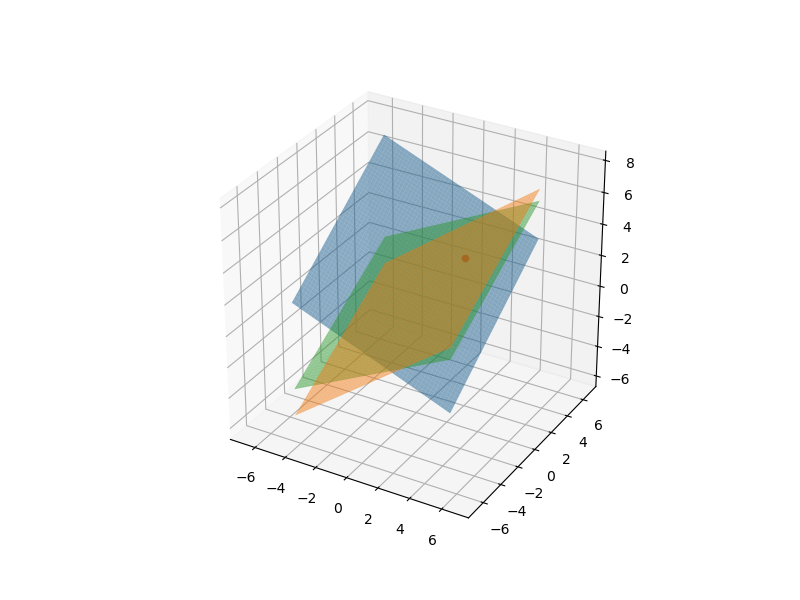
\includegraphics[width=0.8\columnwidth]{figs/img.png}
\caption*{}
\end{figure}

\end{document}
